% Options for packages loaded elsewhere
% Options for packages loaded elsewhere
\PassOptionsToPackage{unicode}{hyperref}
\PassOptionsToPackage{hyphens}{url}
\PassOptionsToPackage{dvipsnames,svgnames,x11names}{xcolor}
%
\documentclass[
  11pt,
]{article}
\usepackage{xcolor}
\usepackage[margin=1in]{geometry}
\usepackage{amsmath,amssymb}
\setcounter{secnumdepth}{-\maxdimen} % remove section numbering
\usepackage{iftex}
\ifPDFTeX
  \usepackage[T1]{fontenc}
  \usepackage[utf8]{inputenc}
  \usepackage{textcomp} % provide euro and other symbols
\else % if luatex or xetex
  \usepackage{unicode-math} % this also loads fontspec
  \defaultfontfeatures{Scale=MatchLowercase}
  \defaultfontfeatures[\rmfamily]{Ligatures=TeX,Scale=1}
\fi
\usepackage{lmodern}
\ifPDFTeX\else
  % xetex/luatex font selection
  \setmainfont[]{Palatino}
\fi
% Use upquote if available, for straight quotes in verbatim environments
\IfFileExists{upquote.sty}{\usepackage{upquote}}{}
\IfFileExists{microtype.sty}{% use microtype if available
  \usepackage[]{microtype}
  \UseMicrotypeSet[protrusion]{basicmath} % disable protrusion for tt fonts
}{}
\makeatletter
\@ifundefined{KOMAClassName}{% if non-KOMA class
  \IfFileExists{parskip.sty}{%
    \usepackage{parskip}
  }{% else
    \setlength{\parindent}{0pt}
    \setlength{\parskip}{6pt plus 2pt minus 1pt}}
}{% if KOMA class
  \KOMAoptions{parskip=half}}
\makeatother
% Make \paragraph and \subparagraph free-standing
\makeatletter
\ifx\paragraph\undefined\else
  \let\oldparagraph\paragraph
  \renewcommand{\paragraph}{
    \@ifstar
      \xxxParagraphStar
      \xxxParagraphNoStar
  }
  \newcommand{\xxxParagraphStar}[1]{\oldparagraph*{#1}\mbox{}}
  \newcommand{\xxxParagraphNoStar}[1]{\oldparagraph{#1}\mbox{}}
\fi
\ifx\subparagraph\undefined\else
  \let\oldsubparagraph\subparagraph
  \renewcommand{\subparagraph}{
    \@ifstar
      \xxxSubParagraphStar
      \xxxSubParagraphNoStar
  }
  \newcommand{\xxxSubParagraphStar}[1]{\oldsubparagraph*{#1}\mbox{}}
  \newcommand{\xxxSubParagraphNoStar}[1]{\oldsubparagraph{#1}\mbox{}}
\fi
\makeatother


\usepackage{longtable,booktabs,array}
\usepackage{calc} % for calculating minipage widths
% Correct order of tables after \paragraph or \subparagraph
\usepackage{etoolbox}
\makeatletter
\patchcmd\longtable{\par}{\if@noskipsec\mbox{}\fi\par}{}{}
\makeatother
% Allow footnotes in longtable head/foot
\IfFileExists{footnotehyper.sty}{\usepackage{footnotehyper}}{\usepackage{footnote}}
\makesavenoteenv{longtable}
\usepackage{graphicx}
\makeatletter
\newsavebox\pandoc@box
\newcommand*\pandocbounded[1]{% scales image to fit in text height/width
  \sbox\pandoc@box{#1}%
  \Gscale@div\@tempa{\textheight}{\dimexpr\ht\pandoc@box+\dp\pandoc@box\relax}%
  \Gscale@div\@tempb{\linewidth}{\wd\pandoc@box}%
  \ifdim\@tempb\p@<\@tempa\p@\let\@tempa\@tempb\fi% select the smaller of both
  \ifdim\@tempa\p@<\p@\scalebox{\@tempa}{\usebox\pandoc@box}%
  \else\usebox{\pandoc@box}%
  \fi%
}
% Set default figure placement to htbp
\def\fps@figure{htbp}
\makeatother





\setlength{\emergencystretch}{3em} % prevent overfull lines

\providecommand{\tightlist}{%
  \setlength{\itemsep}{0pt}\setlength{\parskip}{0pt}}



 


\makeatletter
\@ifpackageloaded{caption}{}{\usepackage{caption}}
\AtBeginDocument{%
\ifdefined\contentsname
  \renewcommand*\contentsname{Table of contents}
\else
  \newcommand\contentsname{Table of contents}
\fi
\ifdefined\listfigurename
  \renewcommand*\listfigurename{List of Figures}
\else
  \newcommand\listfigurename{List of Figures}
\fi
\ifdefined\listtablename
  \renewcommand*\listtablename{List of Tables}
\else
  \newcommand\listtablename{List of Tables}
\fi
\ifdefined\figurename
  \renewcommand*\figurename{Figure}
\else
  \newcommand\figurename{Figure}
\fi
\ifdefined\tablename
  \renewcommand*\tablename{Table}
\else
  \newcommand\tablename{Table}
\fi
}
\@ifpackageloaded{float}{}{\usepackage{float}}
\floatstyle{ruled}
\@ifundefined{c@chapter}{\newfloat{codelisting}{h}{lop}}{\newfloat{codelisting}{h}{lop}[chapter]}
\floatname{codelisting}{Listing}
\newcommand*\listoflistings{\listof{codelisting}{List of Listings}}
\makeatother
\makeatletter
\makeatother
\makeatletter
\@ifpackageloaded{caption}{}{\usepackage{caption}}
\@ifpackageloaded{subcaption}{}{\usepackage{subcaption}}
\makeatother
\usepackage{bookmark}
\IfFileExists{xurl.sty}{\usepackage{xurl}}{} % add URL line breaks if available
\urlstyle{same}
\hypersetup{
  pdftitle={Yash Mali},
  colorlinks=true,
  linkcolor={blue},
  filecolor={Maroon},
  citecolor={Blue},
  urlcolor={Blue},
  pdfcreator={LaTeX via pandoc}}


\title{Yash Mali}
\author{}
\date{}
\begin{document}
\maketitle


\textbf{Email:}
\href{mailto:ymali@student.ubc.ca}{\nolinkurl{ymali@student.ubc.ca}}
\textbar{} \href{https://www.linkedin.com/in/yash-mali-ubc}{LinkedIn}
\textbar{} \href{https://github.com/yashm8}{GitHub}

\subsubsection{About}\label{about}

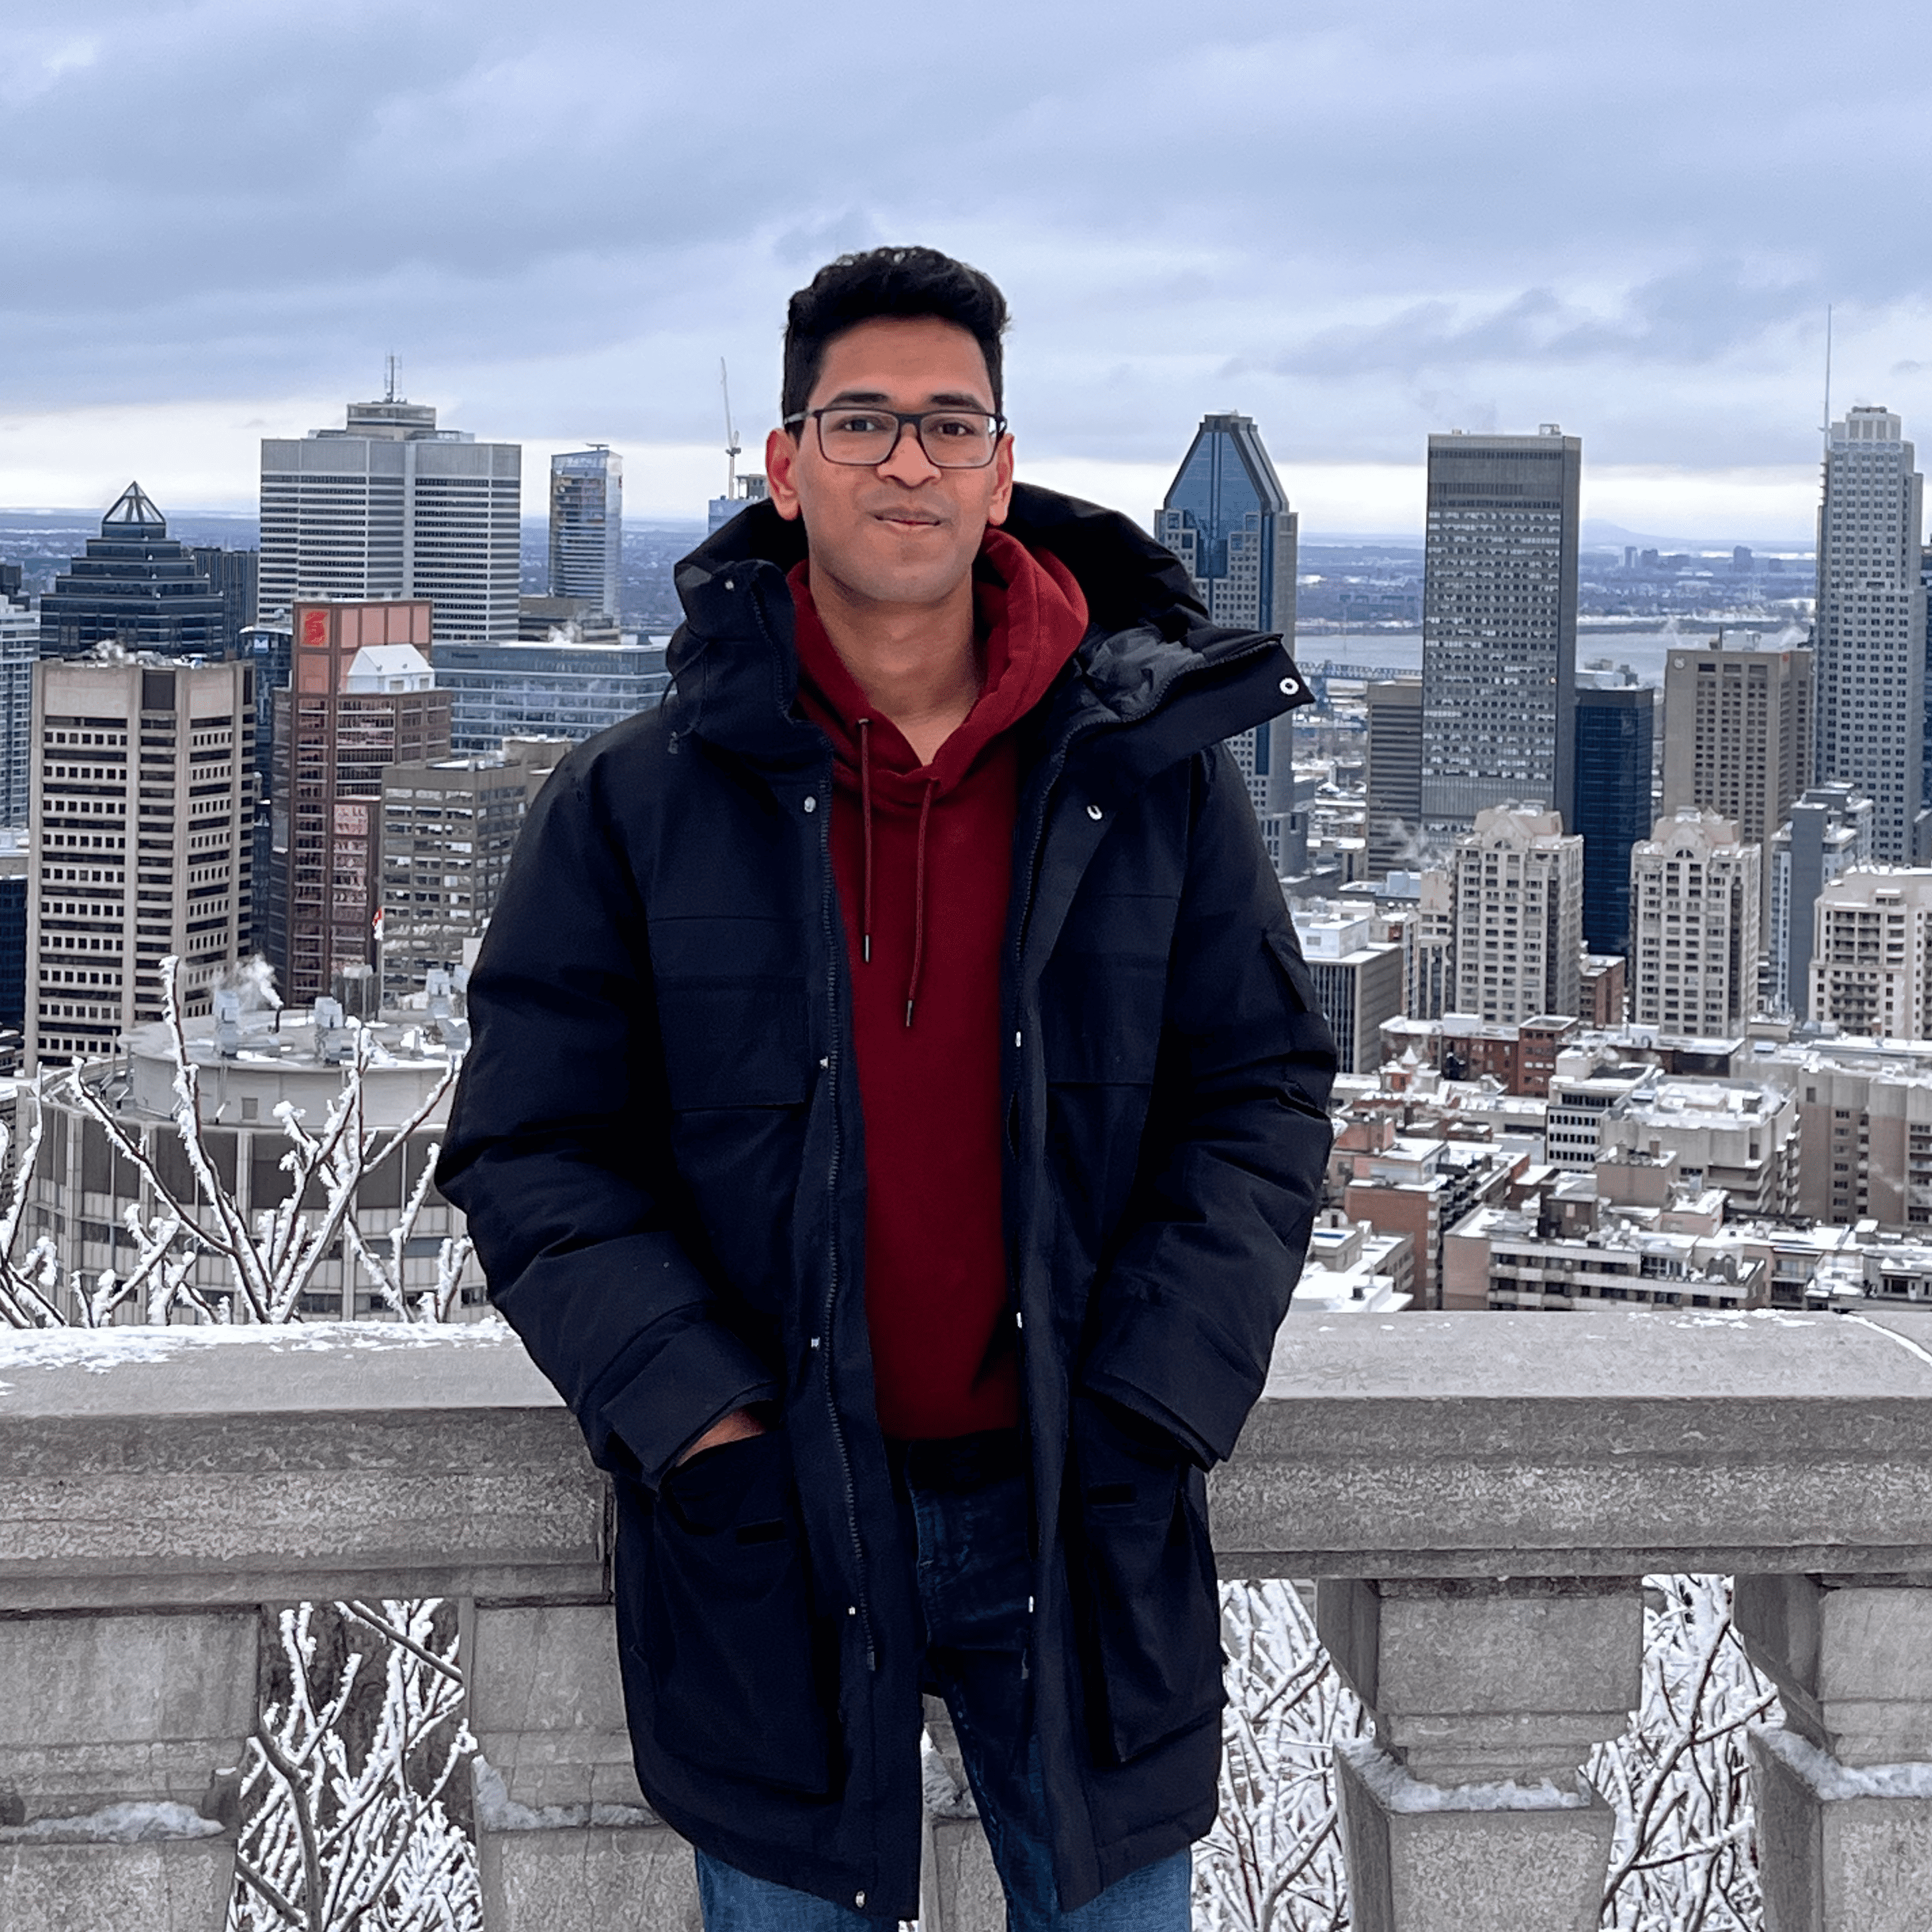
\includegraphics[width=1.5625in,height=\textheight,keepaspectratio]{images/bio-photo.png}

👋🏼 I am an undergraduate student at the University of British Columbia
(UBC) interested in Machine Learning/Artificial Intelligence and
Optimization. I have worked as a Undergraduate Researcher applying AI to
many fields and as a ML engineer. I am driven by fundamental questions
about what deep learning learns and how optimization shapes intelligent
behavior in AI systems.

\subsubsection{Awards}\label{awards}

\href{https://amltn.cs.ubc.ca/people/undergraduate-research-awards}{\textbf{Advanced
Machine Learning Network: AML-TN}}

\emph{April 2025}

\emph{``AML-TN sponsored internships highlight the value of developing
young researchers as the next generation of machine learning
specialists.''}

\href{https://students.ubc.ca/career/ubc-experiences/work-learn-international-undergraduate-research-awards/}{\textbf{2X
Undergraduate Research Award: WLIURA}}

\emph{May 2024, 2025}

\emph{``These awards subsidize professors to hire international
undergraduate students to work full-time on their research projects in
the Summer Session (May to August).''}

\subsubsection{Experience}\label{experience}

\begin{itemize}
\item
  \textbf{Healthcare AI -- Undergraduate Research 🩺} \textbar{}
  \textbf{UBC Medicine} (co-op) \textbar{} \emph{May 2025 -- Sep 2025
  (Continuing part-time)}

  Bringing safe and interpretable AI into medicine. We build software
  that ingests medical guidelines and delivers evidence-based
  recommendations through natural language interfaces, with privacy
  preserved. Our work combines computer science, medical, and clinical
  research in collaboration with UBC's \href{https://cic.ubc.ca/}{Cloud
  Innovation Centre}. Current projects include agentic NLP pipelines
  with UIs hosted on AWS chatbots for Bipolar Disorder and Depression.
  Supervised by
  \href{https://www.google.com/search?q=john+jose+nunez}{Dr.~John Jose
  Nunez}.
\item
  \textbf{ML Engineer -- Undergraduate Research 🏡} \textbar{}
  \textbf{UBC SCARP \& ECE} (part-time) \textbar{} \emph{May 2025 --
  Present}

  Using latest developments in NLP and Computer Vision to analyze public
  records from Vancouver's housing development approval process. This
  work bridges AI and social science to address Canada's housing crisis.
  Supervised by
  \href{https://scarp.ubc.ca/directory/julia-harten}{Dr.~Julia Harten}
  and \href{https://ece.ubc.ca/christos-thrampoulidis/}{Dr.~Christos
  Thrampoulidis}.
\item
  \textbf{Unpacking AI 🎨} \textbar{} \textbf{UBC Arts} (part-time)
  \textbar{} \emph{May 2025 -- Present}

  Developing modules in existing faculty of arts courses that highlight
  how AI can be used in their field. For example, sequence modelling in
  economics or computer vision in archeology. Funded by UBC's Teaching
  and Learning Enhancement fund (TELF). Supervised by
  \href{https://sociology.ubc.ca/profile/laura-nelson/}{Dr.~Laura
  Nelson} and
  \href{https://economics.ubc.ca/profile/jonathan-graves/}{Dr.~Jonathan
  Graves}. \href{https://github.com/ubcecon/praxis-ubc}{More info}.
\item
  \textbf{AI and Automation Developer 🧬} \textbar{}
  \href{https://www.luxbio.ca/}{\textbf{Lux Bio}} (co-op) \textbar{}
  \emph{Sep 2024 -- May 2025}

  Applied AI-based drug discovery tools like AlphaFold and ProteinMPNN
  to optimize sequences and 3D structures of enzymes. Revamped
  automation systems for bioprocess engineering, orchestrating sensors,
  pumps, motors, and valves.
\item
  \textbf{Computer Vision \& Automation -- Undergraduate Research 🔬}
  \textbar{} \textbf{UBC Engineering} @
  \href{https://food.chbe.ubc.ca/}{\textbf{Frostad Research Group}}
  (co-op) \textbar{} \emph{May 2024 -- Sep 2024}

  Developed particle tracking software using an ensemble of open-source
  computer vision models along with a UI to correct mistakes. Automated
  and developed data collection software for new instruments invented by
  the research group. Helped with some day-to-day lab activities.
  Supervised by \href{https://chbe.ubc.ca/john-m-frostad/}{Dr.~John
  Frostad}.
\end{itemize}

\subsubsection{Additional Experience}\label{additional-experience}

\begin{itemize}
\item
  \textbf{\href{https://ubcaiclub.github.io/}{UBC AI Club} 🦾}
  \textbar{} \emph{Jan 2025 -- Present}

  President: Leading initiatives to encourage student understanding and
  future pathways in AI and ML.
\item
  \textbf{\href{https://ubcuas.com/}{UBC Uncrewed Aircraft Systems} ✈️}
  \textbar{} \emph{Sep 2024 -- Present}

  Leading the ML sub-team to explore and tune open-sourced models for
  object detection and tracking. This is a small piece of the puzzle on
  our drones that compete in two university-level autonomous drone
  competitions every year.
\item
  \textbf{\href{https://ubcbiot.com/}{UBC Biological Internet of Things}
  🧬} \textbar{} \emph{May 2025 -- Present}

  Automating brewing/fermentation equipment with IoT-controlled devices
  while also trying to make glow-in-the-dark beer using green
  fluorescent protein (GFP).
\item
  \textbf{\href{https://it.ubc.ca/}{IT Helpdesk Support} 👨‍💻} \textbar{}
  \emph{May 2023 -- May 2024}

  Provided technical assistance to faculty, staff, and students for
  tech-related queries and equipment across campus.
\end{itemize}

\subsection{Selected Work}\label{selected-work}

\subsubsection{Selected Work}\label{selected-work-1}

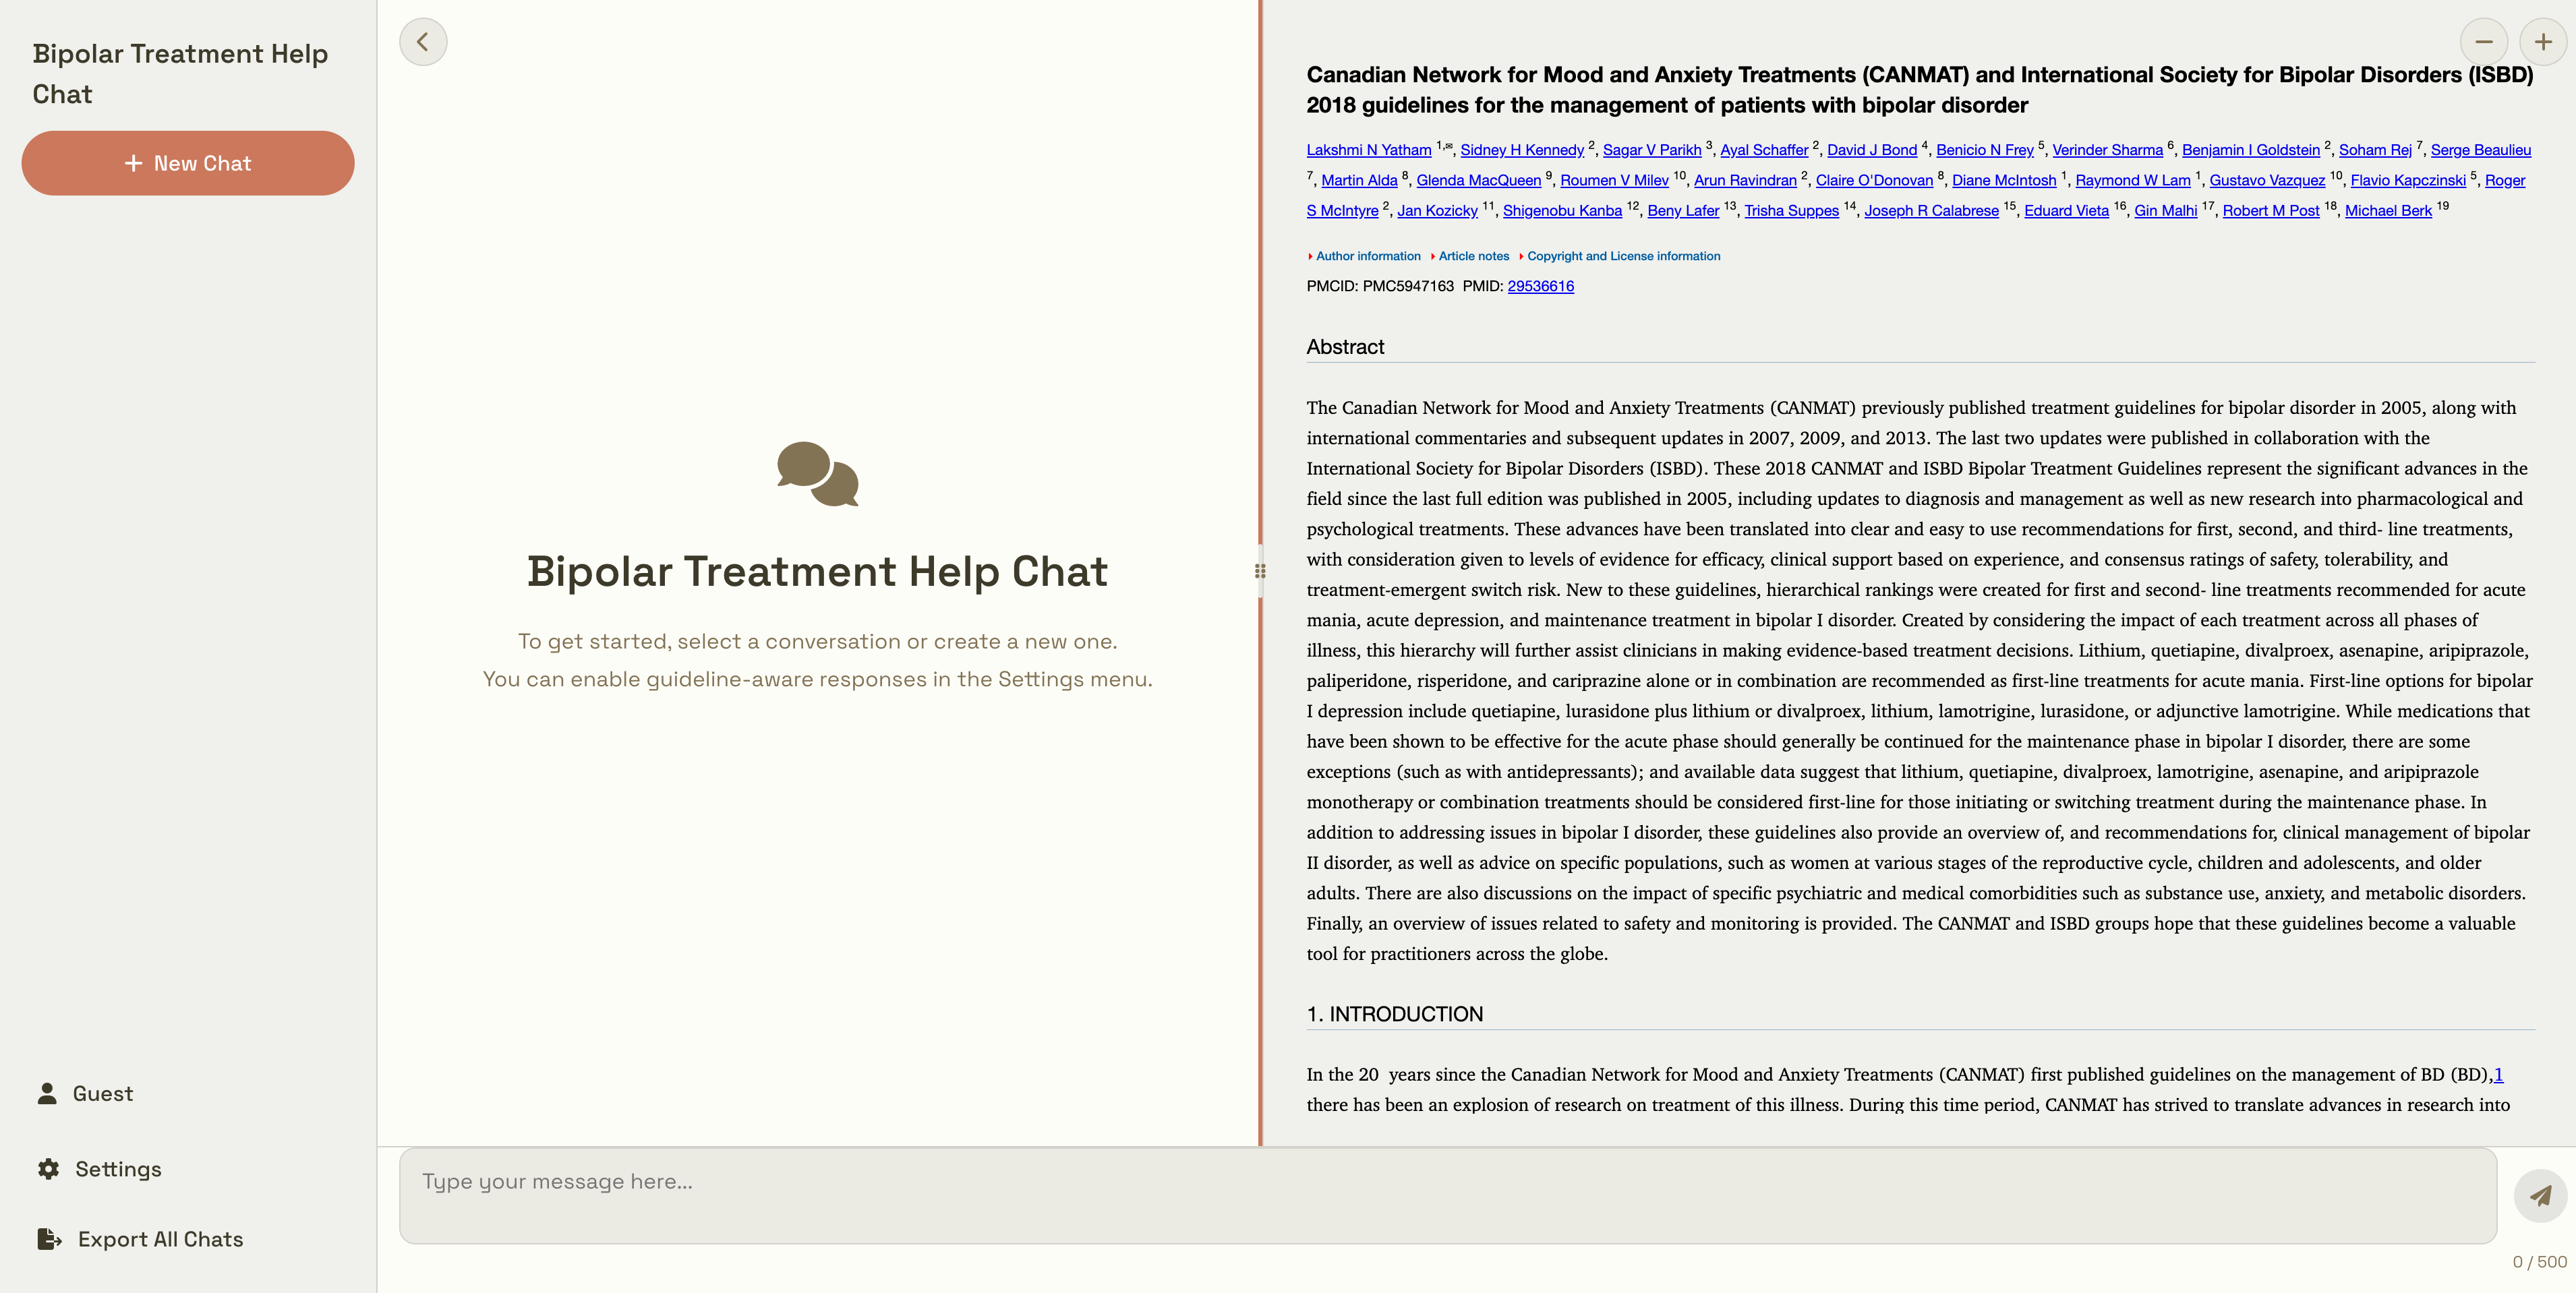
\includegraphics[width=1.5625in,height=\textheight,keepaspectratio]{images/canmat_nlp.png}

\textbf{Agentic NLP for Medical Guidelines}

Poster:
\href{https://caida.ubc.ca/event/poster-session-caidatrustml-2025-icml-visits}{CAIDA/TrustML
ICML Visits 2025} \textbar{} \emph{July 15, 2025}

Poster: \href{https://psychiatry.ubc.ca/2025-eposter-gallery/}{UBC
Psychiatry Research Day 2025} \textbar{} \emph{June 5, 2025}

Talk:
\href{https://students.ubc.ca/career/events-workshops/multidisciplinary-undergraduate-research-conference/}{Multidisciplinary
Undergraduate Research Conference 2025} \textbar{} \emph{Mar 21, 2025}

\begin{center}\rule{0.5\linewidth}{0.5pt}\end{center}

\includegraphics[width=1.5625in,height=\textheight,keepaspectratio]{images/praxis.gif}

\textbf{Praxis UBC: Developing AI education modules in Faculty of Arts
Courses}

Website: \href{https://ubcecon.github.io/praxis-ubc/}{here}

\begin{center}\rule{0.5\linewidth}{0.5pt}\end{center}

\includegraphics[width=1.5625in,height=\textheight,keepaspectratio]{images/starch.png}

\textbf{Quantification of Starch Gelatinization Properties in Glucose
and Sucrose Solutions using ParCS and Deep Learning}

Talk:
\href{https://students.ubc.ca/career/events-workshops/multidisciplinary-undergraduate-research-conference/}{Multidisciplinary
Undergraduate Research Conference 2025} \textbar{} \emph{Mar 21, 2025}

\subsubsection{Small Projects \& Blog}\label{small-projects-blog}

\begin{itemize}
\item
  \textbf{\href{https://yashm8.github.io/dino3.html}{Visualizing DINO v3
  Features}}: Visualize features from a large scale self-supervised
  vision transformer (DINO v3).
\item
  \textbf{\href{https://yashm8.github.io/neural-vis.html}{Visualize how
  Neural Network's move data}}: Visualizing how a small neural network
  transforms toy data.
\end{itemize}




\end{document}
